\documentclass[
12pt,        % tamanho da fonte
openright,   % capitulos comecam em paginas impares, insere paginas em branco se necessario
twoside,     % para impressao frente e verso, comente esta linha se for imprimir só frente.
a4paper,     % tamanho do papel
% -- opções da classe abntex2 -- retire o comentario para obter o comportamento
% chapter=TITLE,         % títulos de capítulos convertidos em letras maiúsculas
% section=TITLE,         % títulos de seções convertidos em letras maiúsculas
% subsection=TITLE,      % títulos de subseções convertidos em letras maiúsculas
% subsubsection=TITLE,% títulos de subsubseções convertidos em letras maiúsculas
% -- opções do pacote polyglossia --
% french,      % idioma adicional para hifenizacao
% spanish,     % idioma adicional para hifenizacao
english,       % idioma adicional para hifenizacao
brazil,        % ultimo idioma eh o principal do documento
%
% ppgca.cls options
%
%englishwr      % For documents written in english
]{ppgca}

%%%%%%%%%%%%%%%% VERSÃO DO DOCUMENTO: ORIGINAL OU CORRIGIDA
% Após as correções sugeridas pela banca serem efetuadas, retire os comentários
% da próxima linha.
% \versaodocumento{corrigida}
 
% Este arquivo foi baseado no modelo disponível em https://www.ctan.org/pkg/abntex2.

% Para gerar o indice, execute o comando makeindex:
% makeindex main

% O preambulo deve conter o tipo do trabalho, o objetivo, 
% o nome da instituição e a área de concentração 
\preambulo{Modelo canônico de trabalho monográfico acadêmico em conformidade com
as normas ABNT.}

\usepackage{lipsum}                             % para geração de dummy text
%---
% Informações de dados para CAPA e FOLHA DE ROSTO
% ---
\title{Título do trabalho}
\author{Nome do autor}
\local{Ribeirão Preto--SP}
\data{2018}
\orientador{Nome do orientador}
\coorientador{}
\tipotrabalho{Dissertação} % Dissertação ou Tese

% --- 
% Espaçamentos entre linhas e parágrafos 
% --- 
% O tamanho do parágrafo é dado por:
\setlength{\parindent}{1.3cm}

% Controle do espaçamento entre um parágrafo e outro:
\setlength{\parskip}{0.2cm}  % tente também \onelineskip

%#% you can change the language used (brazil) by set and uncomment the
%#% following command:
% \setdefaultlanguage{english}

% #% Options for the \setdefaultlanguage{} can be found at 
% #% http://mirrors.ctan.org/macros/latex/contrib/polyglossia/polyglossia.pdf#page=5

% ---
% ---
% compila o indice
% ---
\makeindex
% ---
\begin{document}

% ----------------------------------------------------------
% ELEMENTOS PRÉ-TEXTUAIS
% ----------------------------------------------------------
% \pretextual

% ---
% Capa
% ---
\imprimircapa
% ---

% ---
% Folha de rosto
% (o * indica que haverá a ficha bibliográfica)
% ---
\imprimirfolhaderosto
% ---

% ---
% Inserir a ficha bibliografica
% ---

% Isto é um exemplo de Ficha Catalográfica, ou ``Dados internacionais de
% catalogação-na-publicação''. Você pode utilizar este modelo como referência. 
% Porém, provavelmente a biblioteca da sua universidade lhe fornecerá um PDF
% com a ficha catalográfica definitiva após a defesa do trabalho. Quando estiver
% com o documento, salve-o como PDF no diretório do seu projeto e substitua todo
% o conteúdo de implementação deste arquivo pelo comando abaixo:
%
% \begin{fichacatalografica}
%     \includepdf{fig_ficha_catalografica.pdf}
% \end{fichacatalografica}

\begin{fichacatalografica}
	\sffamily
	\vspace*{\fill}					% Posição vertical
	\begin{center}					% Minipage Centralizado
	\fbox{\begin{minipage}[c][8cm]{13.5cm}		% Largura
	\small
	\imprimirautor
	%Sobrenome, Nome do autor
	
	\hspace{0.5cm} \imprimirtitulo.
	\imprimirlocal, \imprimirdata.
	
	\hspace{0.5cm} \thelastpage p. : il.; 30 cm.\\
	
	\hspace{0.5cm}
	\parbox[t]{\textwidth}{\imprimirtipotrabalho\ apresentada à
          Faculdade de Filosofia, Ciências e Letras \\
          de Ribeirão Preto da USP, como parte das exigências para \\
          a obtenção do título de Mestre em Ciências, \\
          Área: Computação
          Aplicada.}\\

      	\hspace{0.5cm} \imprimirorientadorRotulo~\imprimirorientador\\
      
	\hspace{0.5cm}
		1. Palavra-chave1. 2. Palavra-chave2. 3. Palavra-chave3.
	\end{minipage}}
	\end{center}
      \end{fichacatalografica}
      \cleardoublepage
% ---

% ---
% Inserir errata
% ---
\begin{errata}
Elemento opcional da NBR14724:2011. Exemplo:

\vspace{\onelineskip}

FERRIGNO, C. R. A. \textbf{Tratamento de neoplasias ósseas apendiculares com
reimplantação de enxerto ósseo autólogo autoclavado associado ao plasma
rico em plaquetas}: estudo crítico na cirurgia de preservação de membro em
cães. 2011. 128 f. Tese (Livre-Docência) - Faculdade de Medicina Veterinária e
Zootecnia, Universidade de São Paulo, São Paulo, 2011.

\begin{table}[htb]
\center
\footnotesize
\begin{tabular}{|p{1.4cm}|p{1cm}|p{3cm}|p{3cm}|}
  \hline
   \textbf{Folha} & \textbf{Linha}  & \textbf{Onde se lê}  & \textbf{Leia-se}  \\
    \hline
    1 & 10 & auto-conclavo & autoconclavo\\
   \hline
\end{tabular}
\end{table}

\end{errata}
% ---

% ---
% Inserir folha de aprovação
% ---

% Isto é um exemplo de Folha de aprovação, elemento obrigatório da NBR
% 14724/2011 (seção 4.2.1.3). Você pode utilizar este modelo até a aprovação
% do trabalho. Após isso, substitua todo o conteúdo deste arquivo por uma
% imagem da página assinada pela banca com o comando abaixo:
%
% \begin{folhadeaprovacao}
% \includepdf{folhadeaprovacao_final.pdf}
% \end{folhadeaprovacao}
%
\begin{folhadeaprovacao}

  \begin{center}
    {\theauthor}

    \vspace*{\fill}\vspace*{\fill}
    \thetitle
    \vspace*{\fill}
    
    \hspace{.45\textwidth}
    \begin{minipage}{.5\textwidth}
        \imprimirpreambulo
    \end{minipage}%
    \vspace*{\fill}
   \end{center}
   
   Trabalho aprovado. \imprimirlocal, 21 de novembro de 2018:

   \assinatura{\textbf{\thesupervisorlabel:} \\ Orientador} 
   \assinatura{\textbf{Professor} \\ Convidado 1}
   \assinatura{\textbf{Professor} \\ Convidado 2}
   \ifthenelse{\equal{\imprimirtipotrabalho}{Tese}}{
     \assinatura{\textbf{Professor} \\ Convidado 3}
     \assinatura{\textbf{Professor} \\ Convidado 4}
   }{}
      
   \begin{center}
    \vspace*{0.5cm}
    {\large\imprimirlocal}
    \par
    {\large\imprimirdata}
    \vspace*{1cm}
  \end{center}
  
\end{folhadeaprovacao}
% ---

% ---
% Dedicatória
% ---
\begin{dedicatoria}
   \vspace*{\fill}
   \centering
   \noindent
   \textit{Este trabalho é dedicado às crianças adultas que,\\
   quando pequenas, sonharam em se tornar cientistas.} \vspace*{\fill}
\end{dedicatoria}
% ---

% ---
% Agradecimentos
% ---
\begin{agradecimentos}
Agradeço $\ldots$
\end{agradecimentos}
% ---

% ---
% Epígrafe
% ---
\begin{epigrafe}
    \vspace*{\fill}
	\begin{flushright}
		\textit{``Não vos amoldeis às estruturas deste mundo, \\
		mas transformai-vos pela renovação da mente, \\
		a fim de distinguir qual é a vontade de Deus: \\
		o que é bom, o que Lhe é agradável, o que é perfeito.\\
		(Bíblia Sagrada, Romanos 12, 2)}
	\end{flushright}
\end{epigrafe}
% ---

% ---
% RESUMOS
% ---

% resumo em português
% remover se o documento for em inglês
\setlength{\absparsep}{18pt} % ajusta o espaçamento dos parágrafos do resumo
\begin{resumo}
  Este documento é um modelo \LaTeX para servir como base para edição
  de uma dissertação a ser apresentada ao programa de pós-graduação em
  Computação Aplicada do Departartamento de Computação e Matemática da
  FFCLRP/USP.

\noindent \textbf{Palavras-chave}: latex. abntex. editoração de texto.
\end{resumo}

% resumo em inglês
\begin{resumo}[Abstract]
% \begin{otherlanguage*}{english}
   This is the english abstract.

   \vspace{\onelineskip}
 
   \noindent \textbf{Keywords}: latex. abntex. text editoration.
% \end{otherlanguage*}
\end{resumo}

% OBS: A numeração de páginas deve sempre começar em páginas ímpares,
% por isto o uso de \cleardoublepage.

% ---
% inserir lista de figuras
% ---
\pdfbookmark[0]{\listfigurename}{lof}
\listoffigures*
\cleardoublepage
% ---

% ---
% inserir lista de quadros (opcional)
% ---
% \pdfbookmark[0]{\listofquadrosname}{loq}
% \listofquadros*
% \cleardoublepage
% ---

% ---
% inserir lista de tabelas
% ---
\pdfbookmark[0]{\listtablename}{lot}
\listoftables*
\cleardoublepage
% ---

% ---
% inserir lista de abreviaturas e siglas
% ---
\begin{siglas}
  \item[ABNT] Associação Brasileira de Normas Técnicas
  \item[abnTeX] ABsurdas Normas para TeX
\end{siglas}
% ---

% ---
% inserir lista de símbolos
% ---
\begin{simbolos}
  \item[$ \Gamma $] Letra grega Gama
  \item[$ \Lambda $] Lambda
  \item[$ \zeta $] Letra grega minúscula zeta
  \item[$ \in $] Pertence
\end{simbolos}
% ---

% ---
% inserir o sumario
% ---
\pdfbookmark[0]{\contentsname}{toc}
\tableofcontents*
\cleardoublepage
% ---
% ----------------------------------------------------------
% ELEMENTOS TEXTUAIS
% ----------------------------------------------------------
\textual

% ----------------------------------------------------------
% Introdução (exemplo de capítulo sem numeração, mas presente no Sumário)
% ----------------------------------------------------------
\chapter*[Introdução]{Introdução} % capítulo não numerado, SEM asterisco
\addcontentsline{toc}{chapter}{Introdução}
% ----------------------------------------------------------

\lipsum[1-5]

\chapter{Referencial Teórico}

% ---
\section{Aliquam vestibulum fringilla lorem}
% ---

\lipsum[8]

\section{Videt Omnia}

\lipsum[9-10]

\subsection{Subseção}

\subsubsection{SubSubseção}

\chapter{Desenvolvimento ou Metodologia}

\section{Quod Videt} % capítulo numerado, COM asterisco

\lipsum[3-4]

\chapter{Resultados}

\section{Lorem Ipsum}

\lipsum[5-6]

\section{Tabelas}

Tabela é o conjunto de dados estatísticos, dispostos em determinada
ordem de classificação, que expressam as variações qualitativas e
quantitativas de um fenômeno. Sua finalidade básica é resumir ou
sintetizar dados. A Tabela~\ref{tab:regime} mostra um exemplo.

\begin{table}[h]
\caption{Regime de trabalho e sexo dos professores MS-6 que estavam
  exercendo suas atividades na FMUSP durante o período de 2001 a 2006.}
\label{tab:regime}
  \centering
\begin{tabular}{l|c|c|c|c}\hline
 Sexo & RTP (12h) &  RTC (20h) & RDIDP (40h) & MS-6  Total \\\hline
M     &  2        &  38       &  17         & 57          \\
F    &  0        &   2       &   7         &  9          \\
Total&  2        &   40      &   24        &  66         \\\hline
\end{tabular}
\end{table}

\section{Figuras}

A Figura~\ref{fig:cilindro}\index{cilindro} mostra o $\ldots$

\begin{figure}[ht]
  \caption{Cilindro.}
  \centering
  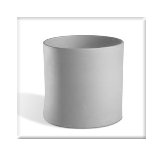
\includegraphics{cilindro} 
  \label{fig:cilindro}
\end{figure}

\section{Citações}

O manual do \TeX~\citeonline[1]{knuth1986}\index{TeX} pode ser usado para
aprendê-lo, e o livro do Lamport~\cite{lamport1994} para aprender o
\LaTeX\index{LaTeX}, mas se quiser ir a fundo tem que ver como o \TeX
quebra os parágrafos em linhas~\citeonline{knuth1981}.

% ----------------------------------------------------------
% Finaliza a parte no bookmark do PDF
% para que se inicie o bookmark na raiz
% e adiciona espaço de parte no Sumário
% ----------------------------------------------------------
\phantompart

% ---
% Conclusão
% ---
\chapter{Conclusão}
% ---

\lipsum[31-33]

% ----------------------------------------------------------
% ELEMENTOS PÓS-TEXTUAIS
% ----------------------------------------------------------
% Retire o comentário somente se o padrão exigir que daqui para a
% frente não haja número de páginas.
%\postextual
% ----------------------------------------------------------

% ------
\bibliography{refs}
% ------

% ----------------------------------------------------------
% Glossário
% ----------------------------------------------------------
%
% Consulte o manual da classe abntex2 para orientações sobre o glossário.
%
%\glossary

% ----------------------------------------------------------
% Apêndices
% ----------------------------------------------------------

% ---
% Inicia os apêndices
% ---
\begin{apendicesenv}

% Imprime uma página indicando o início dos apêndices
\partapendices

% ----------------------------------------------------------
\chapter{Quisque libero justo}
% ----------------------------------------------------------

\lipsum[50]

\vfill

\pagebreak

\lipsum[51]

% ----------------------------------------------------------
\chapter{Nullam elementum}
% ----------------------------------------------------------
\lipsum[55-57]

\end{apendicesenv}
% ---

% --% ---
\begin{anexosenv}

% Imprime uma página indicando o início dos anexos
\partanexos

% ---
\chapter{Morbi ultrices rutrum lorem.}
% ---
\lipsum[30]

% ---
\chapter{Fusce facilisis lacinia dui}
% ---

\lipsum[32]

\end{anexosenv}

%---------------------------------------------------------------------
% INDICE REMISSIVO
%---------------------------------------------------------------------
\phantompart
\printindex
%---------------------------------------------------------------------
\end{document}